\documentclass[a4paper,12pt]{article} 

%%% Работа с русским языком
\usepackage{cmap}                           % поиск в PDF
\usepackage{mathtext} 			 	       % русские буквы в формулах
\usepackage[T2A]{fontenc}               % кодировка
\usepackage[utf8]{inputenc}              % кодировка исходного текста
\usepackage[english,russian]{babel}  % локализация и переносы
\usepackage[left=2cm,right=2cm,
    top=2cm,bottom=3cm,bindingoffset=0cm]{geometry}
\usepackage{wrapfig}
\usepackage{gensymb}
\usepackage{textcomp}
\usepackage{multirow}

\usepackage{pgfplots}
\usepackage{amsmath,amsfonts,amssymb,amsthm,mathtools} % AMS
\usepackage{euscript}	 % Шрифт Евклид
\usepackage{mathrsfs} % Красивый матшрифт
\usepackage{graphicx}%Вставка картинок правильная
\usepackage{float}%"Плавающие" картинки
\usepackage{wrapfig}%Обтекание фигур (таблиц, картинок и прочего)
\title{Лабораторная работа 4.7.2

Эффект Поккельса}
\author{Кагарманов Радмир Б01-106}
\date{19 апреля 2023 г.}

\begin{document}
\maketitle
\thispagestyle{empty}
\newpage
\setcounter{page}{1}

\paragraph{Цель работы:} исследовать интерференцию рассеянного света, прошедшего кристалл; наблюдать изменение характера поляризации света при наложении на кристалл электрического поля.
\paragraph{В работе используется:} гелий-неоновый лазер, поляризатор, кристалл ниобата лития, матовая пластинка, экран, источник высоко-вольтного переменного и постоянного напряжения, фотодиод, осциоллограф, линейка.
\paragraph{Теоретические сведения\\}
Эффект Поккельса -- изменение показателя преломления света в кристалле под действием электрического поля.\par
Рассмотрим кристалл ниобата лития $\text{LiNbO}_3$ с цетрольноосевой симметрией вдоль оси $Z$. Для световой волны с $\mathbf{E}$ перпендикулярно $Z$ показатель преломления будет $n_o$, а для волны с $\mathbf{E}$ вдоль $Z$ -- $n_e$. В случае, когда луч света идёт под углом $\theta$ к оси, есть два значение показателя преломления $n_1$ и $n_2$: $n_1 = n_o$ для волны с $\mathbf{E}$ перпендикулярным плоскости $(\mathbf{k},\mathbf{Z})$ (обыкновенная волна) и $n_2$ для волны с $\mathbf{E}$ в этой плоскости (необыкновенная волна). В последнем случае
\begin{equation}
\dfrac{1}{n_2^2}=\dfrac{\cos^2 \theta}{n_0^2}+\dfrac{\sin^2 \theta}{n_e^2}.
\end{equation}

\begin{wrapfigure}{r}{0.5\textwidth}
\begin{center}
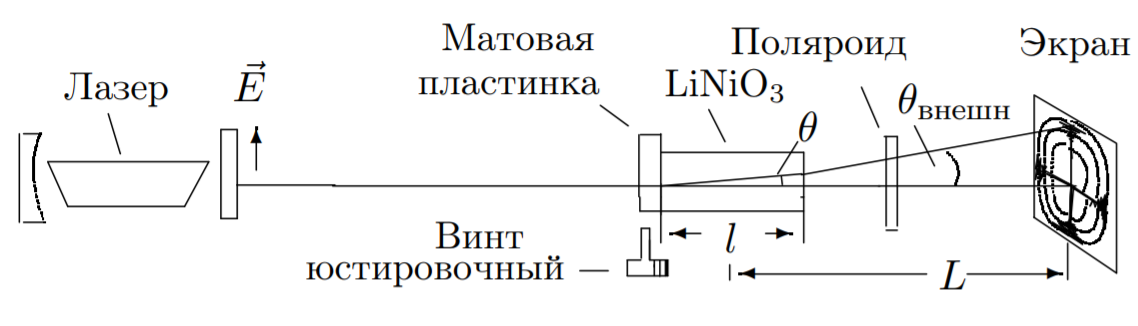
\includegraphics[width = 0.5\textwidth]{1.png}
\end{center}
\vspace{-20pt}
\caption{Схема для наблюдения интерфереционной картины.}
\end{wrapfigure}
%\begin{figure}[h!]
%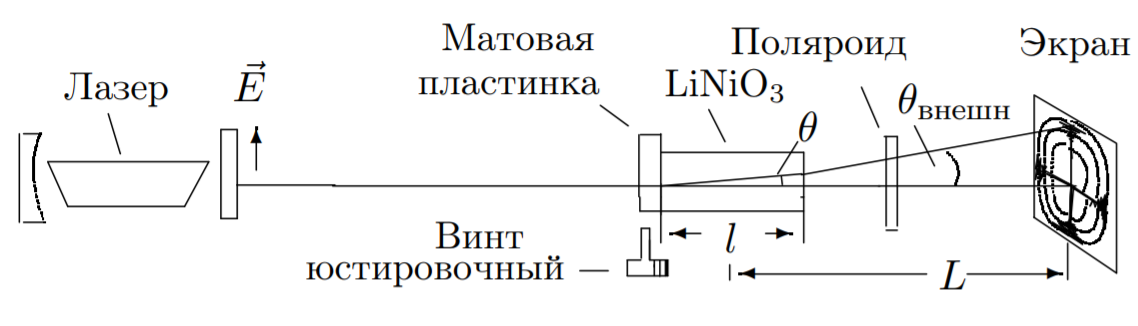
\includegraphics[scale=0.5]{1.png}
%\centering
%\caption{Схема для наблюдения интерфереционной картины}
%\end{figure}
Если перед кристаллом, помещённым между поляроидами, расположить линзу или матовую пластинку, то на экране за поляроидом мы увидим тёмные концентрические окружности -- рещультат интерфернции обыкновенной и необыкновенной волн. При повороте выходного поляроида на $90^\circ$ картина меняется с позитива на негатив (на месте светлых пятен тёмные и наоборот). В случаи, когда разрешённое направление анализатора перпендикулярно поляризации лазерного излучения, радиус тёмного кольца с номером $m$ равен
\begin{equation}
r_m^2 = \dfrac{\lambda}{l} \dfrac{(n_oL)^2}{n_0 - n_e}m,
\end{equation}

\begin{wrapfigure}{r}{0.45\textwidth}
\begin{center}
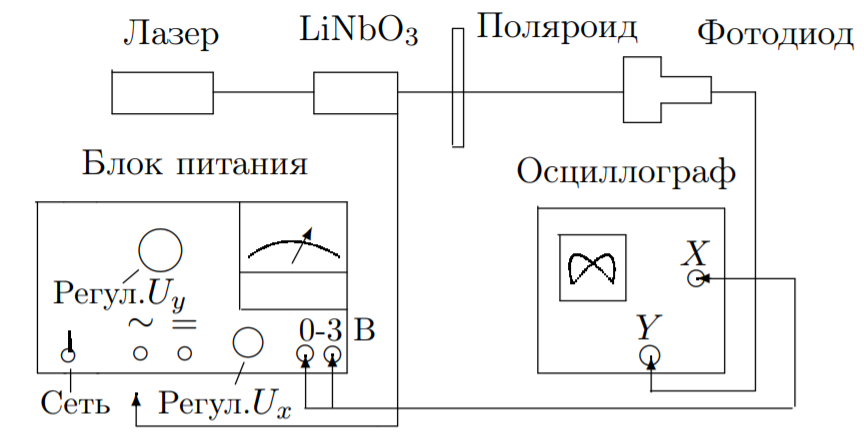
\includegraphics[width = 0.45\textwidth]{2.png}
\end{center}
\vspace{-20pt}
\caption{Схема установки.}
\end{wrapfigure}

где $L$ -- расстояние от центра кристалла до экрана, $l$ -- длина кристалла.\\
Теперь поместим кристалл в постоянное электрическое поле $E_{\text{эл}}$, направленное вдоль оси $X$, перпендикулярной $Z$. Показатель преломления для луча, распространяющего вдоль $Z$, всегда $n_o$. В плоскости $(X,Y)$ возникают два главных направления под углами $45^\circ$ к $X$ и $Y$ с показателями преломления $n_0 - \Delta n$ и $n_o + \Delta n$ (быстрая и медленная ось), причём $\Delta n = A E_{\text{эл}}$. Для поляризованного вертикально света и анализатора, пропускающего горизонтальную поляризацию, на выходе интенсивность на выходе будет иметь вид
\begin{equation}
I_{\text{вых}} = I_0 \sin^2 \left(\dfrac{\pi}{2} \dfrac{U}{U_{\lambda/2}} \right),
\end{equation}
где $U_{\lambda/2} = \frac{\lambda}{4A}\frac{d}{l}$ -- \textit{полуволновое напряжение}, $d$ -- поперечный размер кристалла.  При напряжении $U = E_{\text{эл}}d$ равном полуволновому сдвиг фаз между двумя волнами равен $\pi$, а интенсивность света на выходе максимальна. 


На Рис. 2 представлена схема всей установки (оптическая часть изорбажена на Рис. 1). Свет лазера, проходя через сквозь пластину, рассеивается и падает на двоякопреломляющий кристалл. На экране за поляроидом видна интерференционная картина. Убрав рассеивающую пластину и подавая на кристалл постоянное напряжение, можно величиной напряжения влиять на поляризацию луча, вышедшего из кристалла. Заменив экран фотодиодом и подав на кристалл переменное напряжение, можно исследовать поляризацию с помощью осциллографа.
\paragraph{Обработка результатов}
\subparagraph{1.} Выполним юстировки системы, изображённой на Рис. 1 и получим интерференционное изображение.
\subparagraph{2.} Измерим радиусы тёмных колец при расстоянии $L=82,2\pm 0,1 ~ см$. от середины кристалла до экрана. Результаты в Таблице 1. На Рис. 3 изображён график зависимости $r^2 = f(m)$.

\begin{figure}[h!]
	\centering
	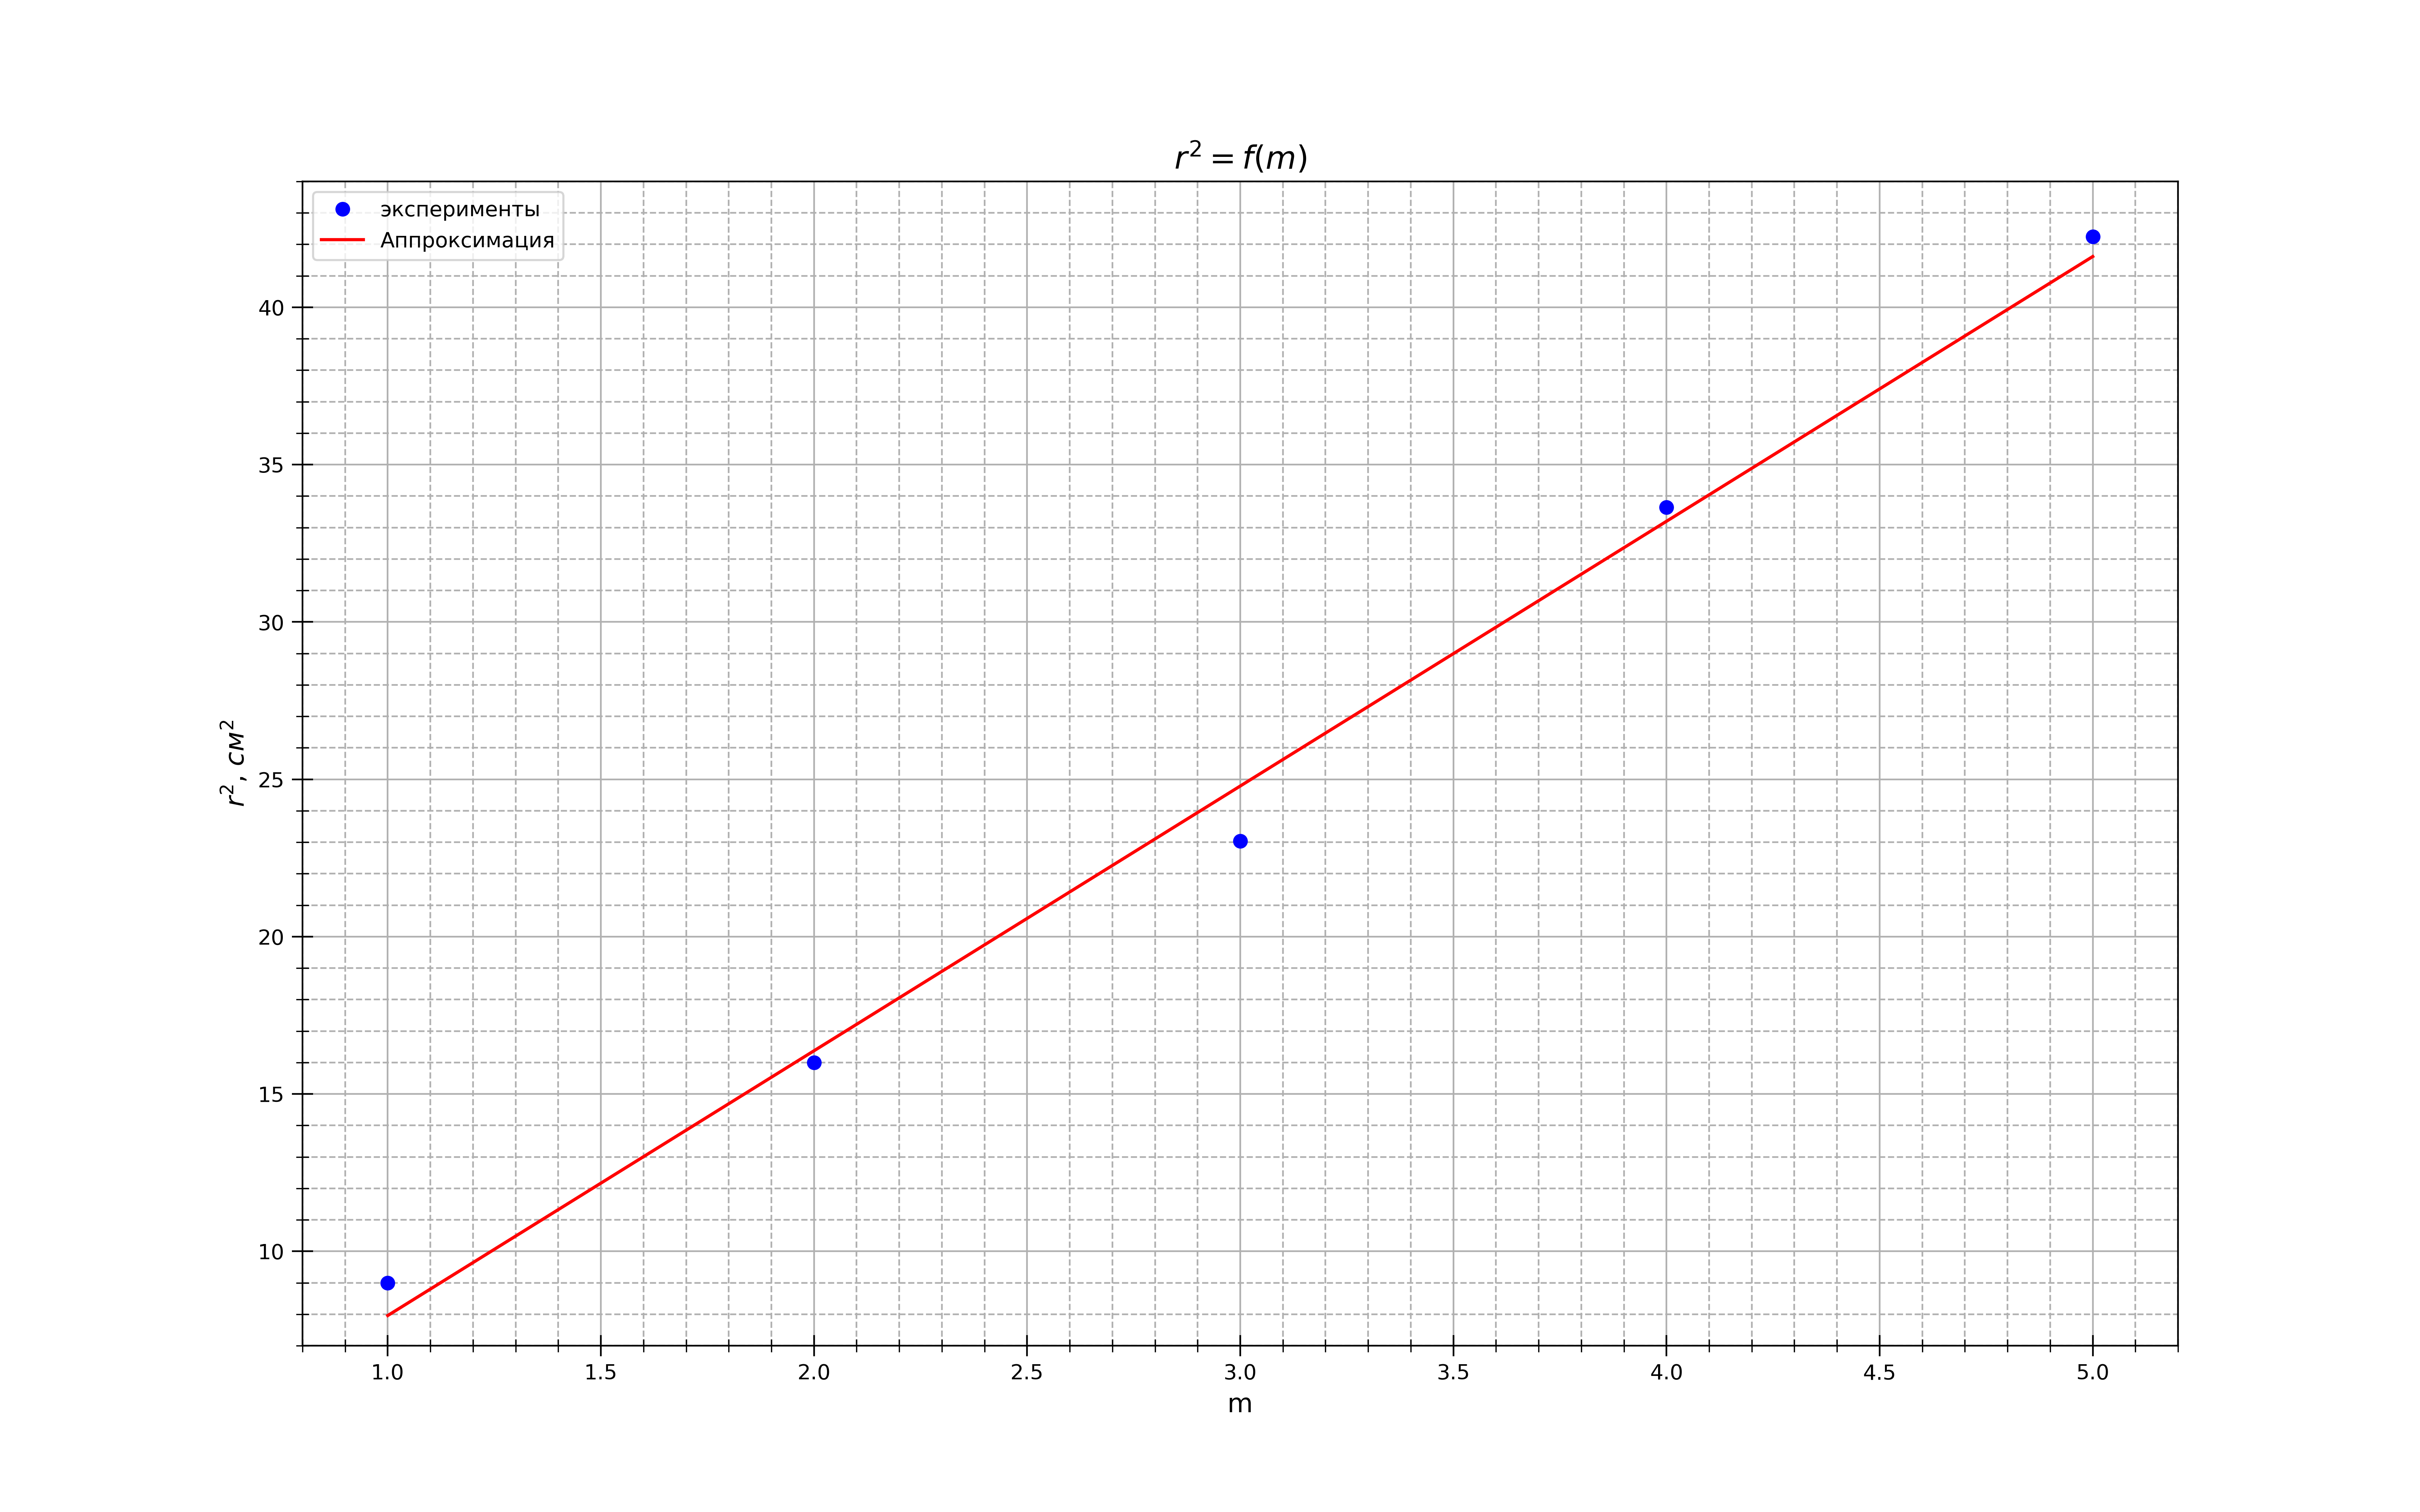
\includegraphics[width=1\linewidth]{graph1.png}
	\caption{$r^2=f(m)$}
	\label{labA}
\end{figure}

Угловой коэффициент $k= 8,4 \pm 0,3 см^2$. Из формулы (2) найдём $n_0-n_e$ для значений: $n_0 = 2,29$, $\lambda = 0,63$ мкм, $l = 26$ мм.

\begin{center}
    $n_0-n_e = 0,102\pm 0,027$
\end{center}

\subparagraph{3.} \par Убедимся ещё раз, что направление лазерного луча совпадает с направлением на центр интерференционной картины и уберём матовую пластинку. Подключим разъём блока питания на постоянно напряжение, установим регулятор напряжения на минимум и включим блок питания в сеть.

Сначала определим интересующие нас напряжения без осциллографа. Для этого уберём матовую пластинку. При нулевом напряжении наблюдается минимум интенсиности излучения на экране. Постепенно увеличивая его, получим напряжение, соответстующее максимуму интенсивности $U_{\lambda/2} = (195 \pm 15) \text{ В}$.

Увеличивая напряжение далее определяем $U_\lambda$:

\[U_\lambda = (420 \pm 15) \text{ В} \]

\par Подадим на кристалл напряжение $U_{\lambda/4} = \frac{1}{2}U_{\lambda/2}$. Вращая анализатор и наблюдая за яркостью пятна на экране, убеждаемся, что поляризация круговая.\par

Дальнейшие измерения проводим при помощи осциллографа. Полуволновое напряжение, измеренное с помощью осциоллографа, совпадает с измеренным ранее. 

Вид фигур Лиссажу для этих напряжений представлен в Таблице 2.

\begin{table}[h]
\centering
\begin{tabular}{|c|c|c|}
\hline
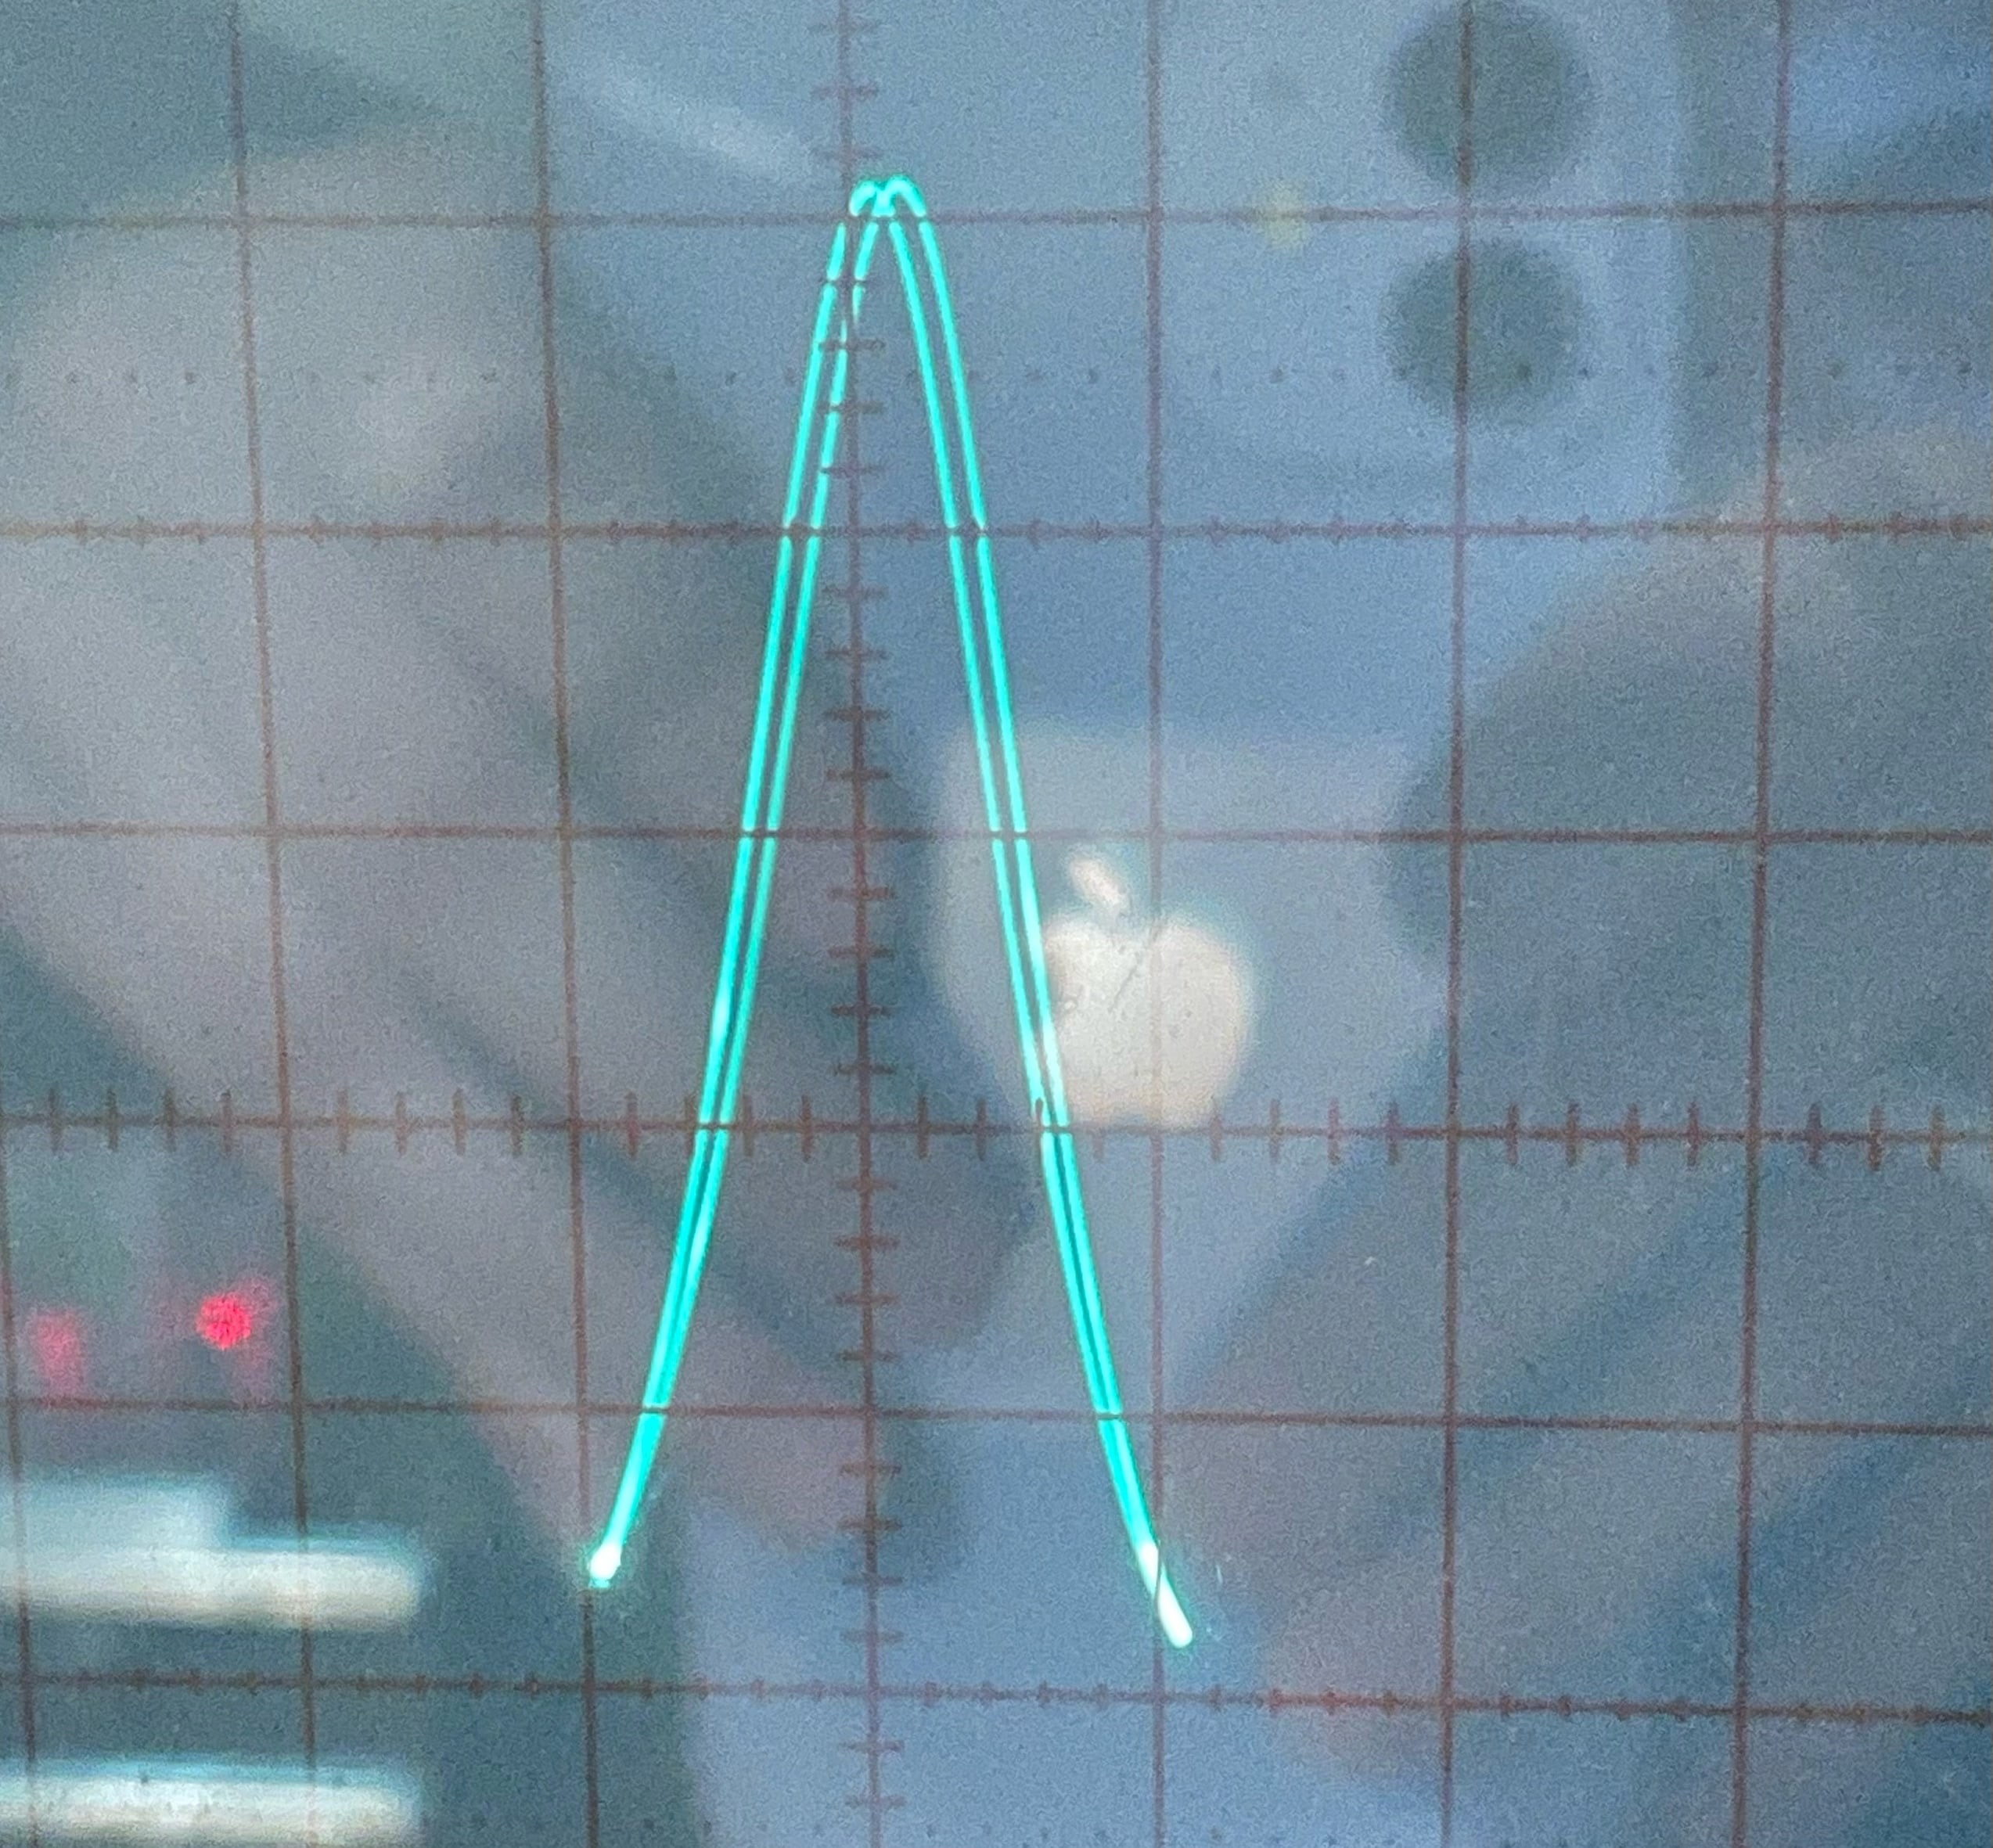
\includegraphics[height=4cm]{liss1.png}  & 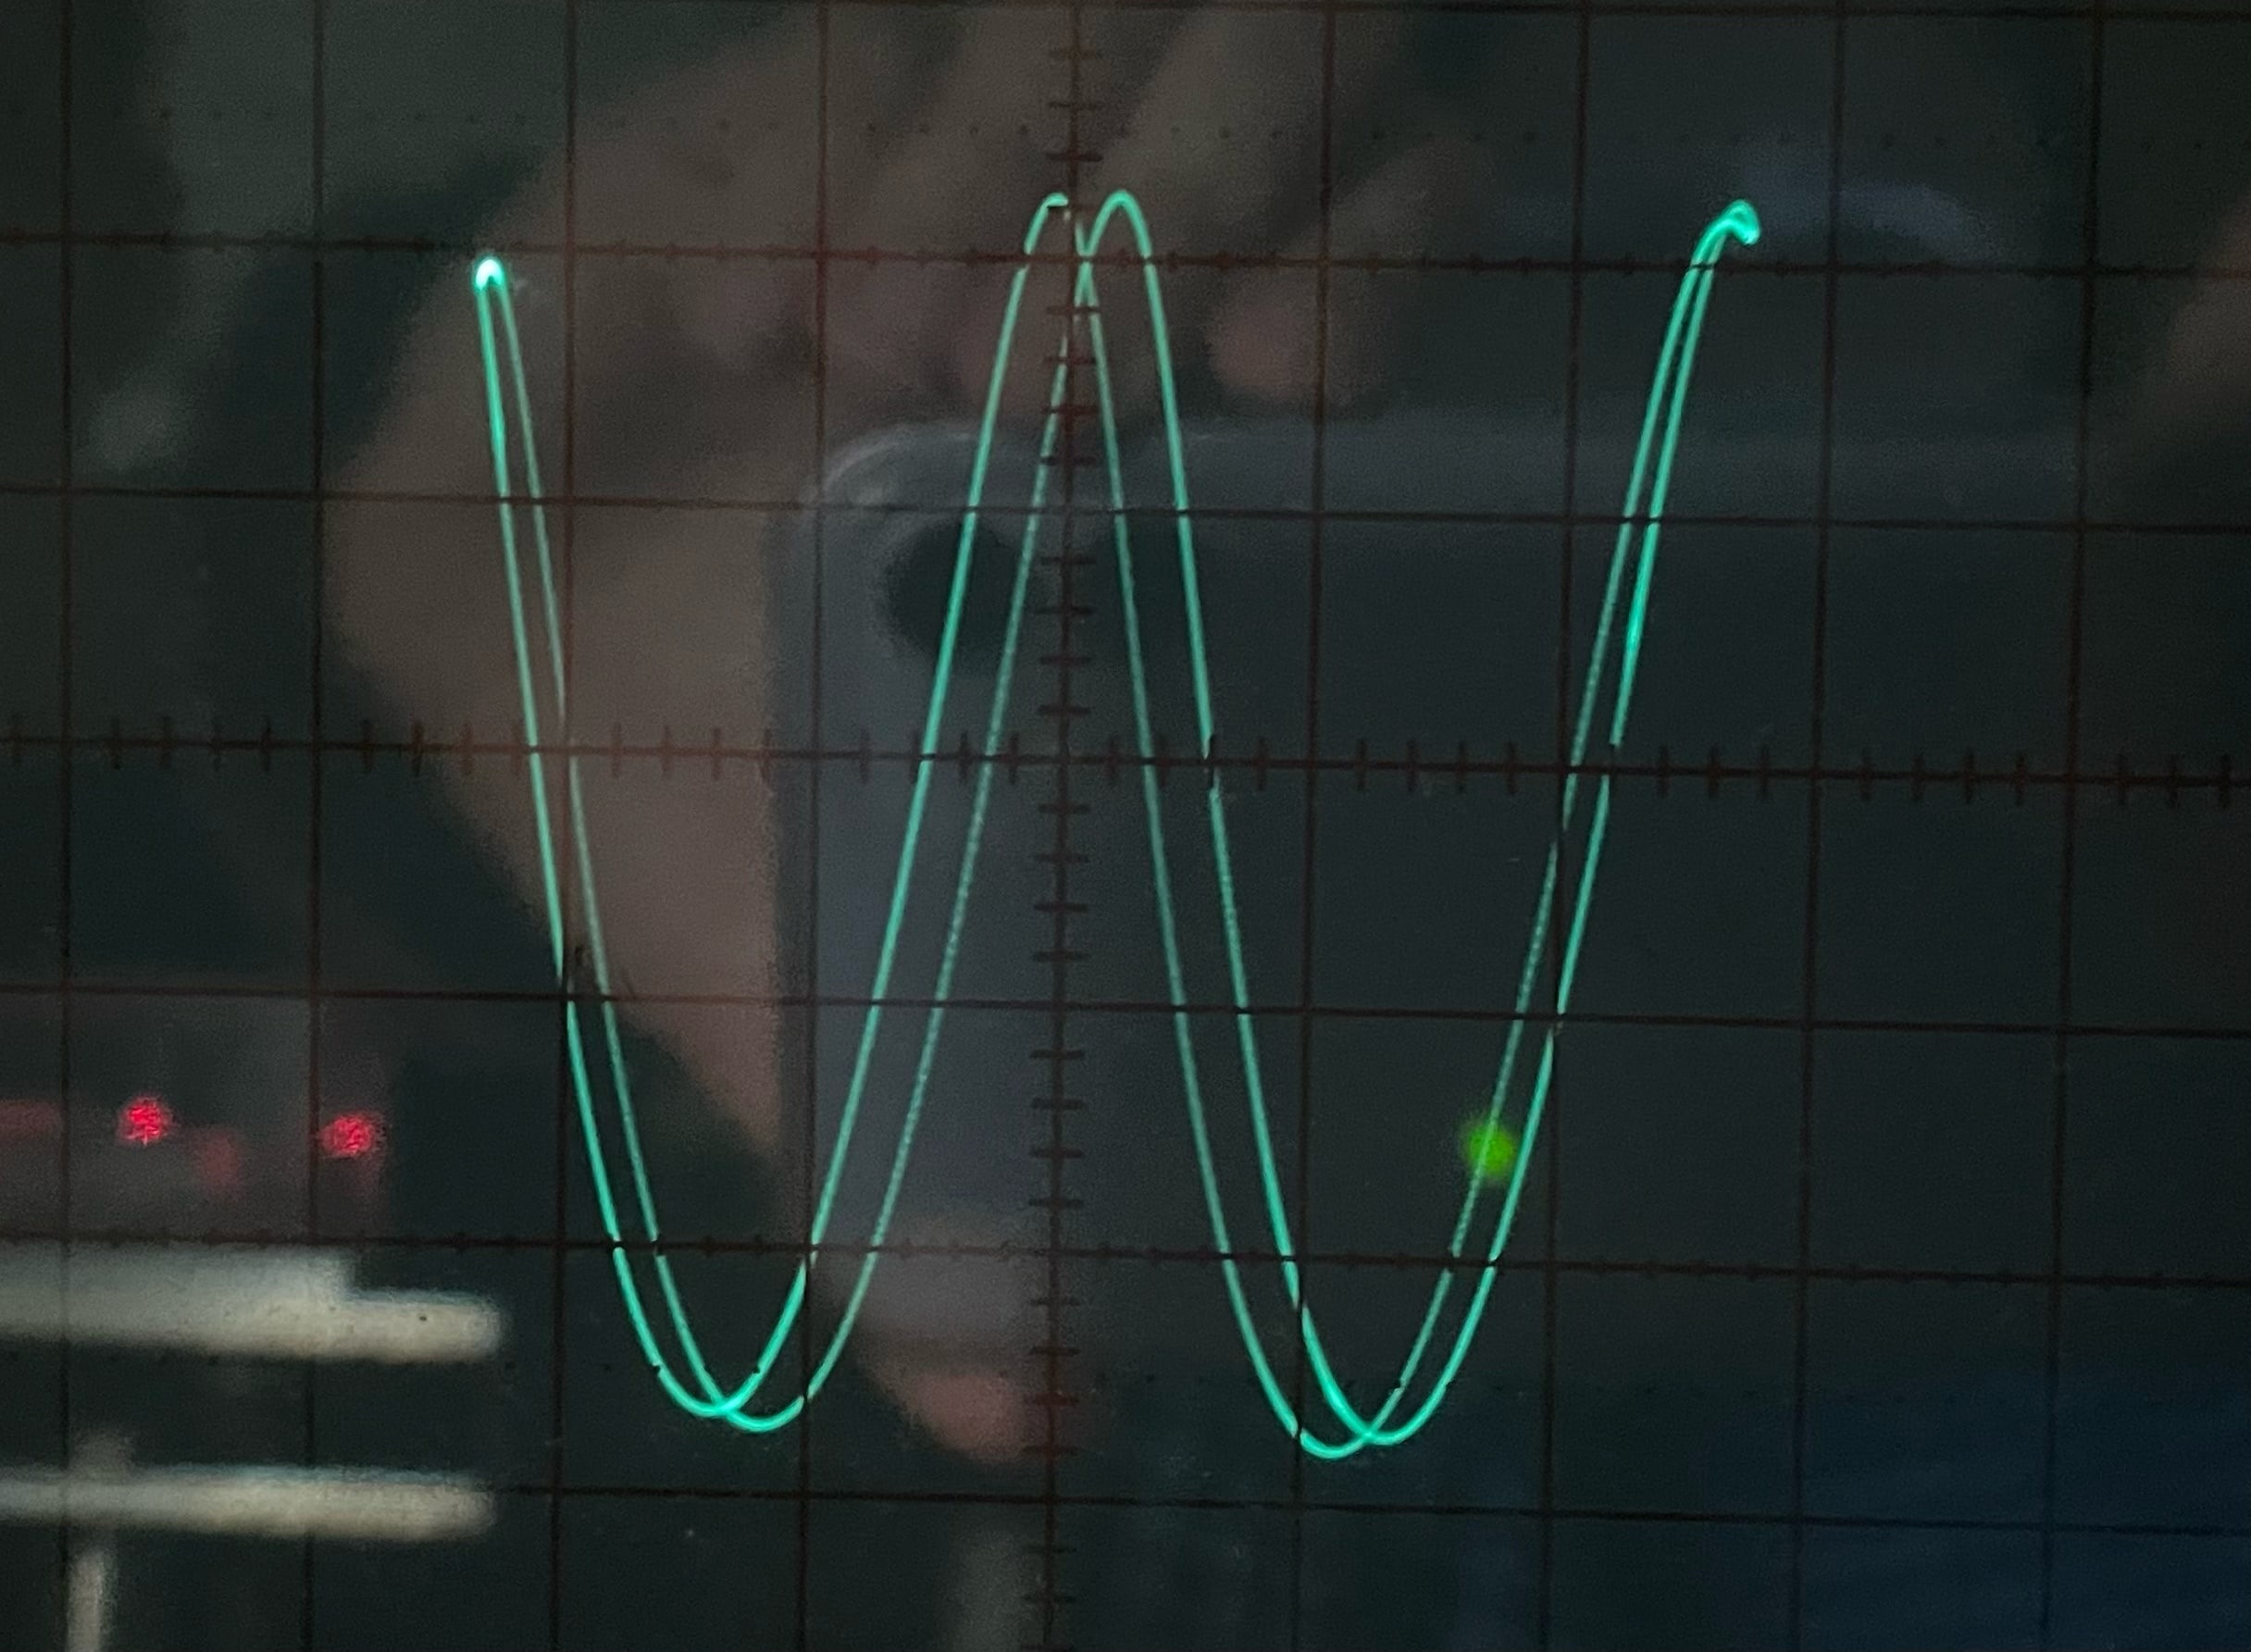
\includegraphics[height=4cm]{liss2.png}  &  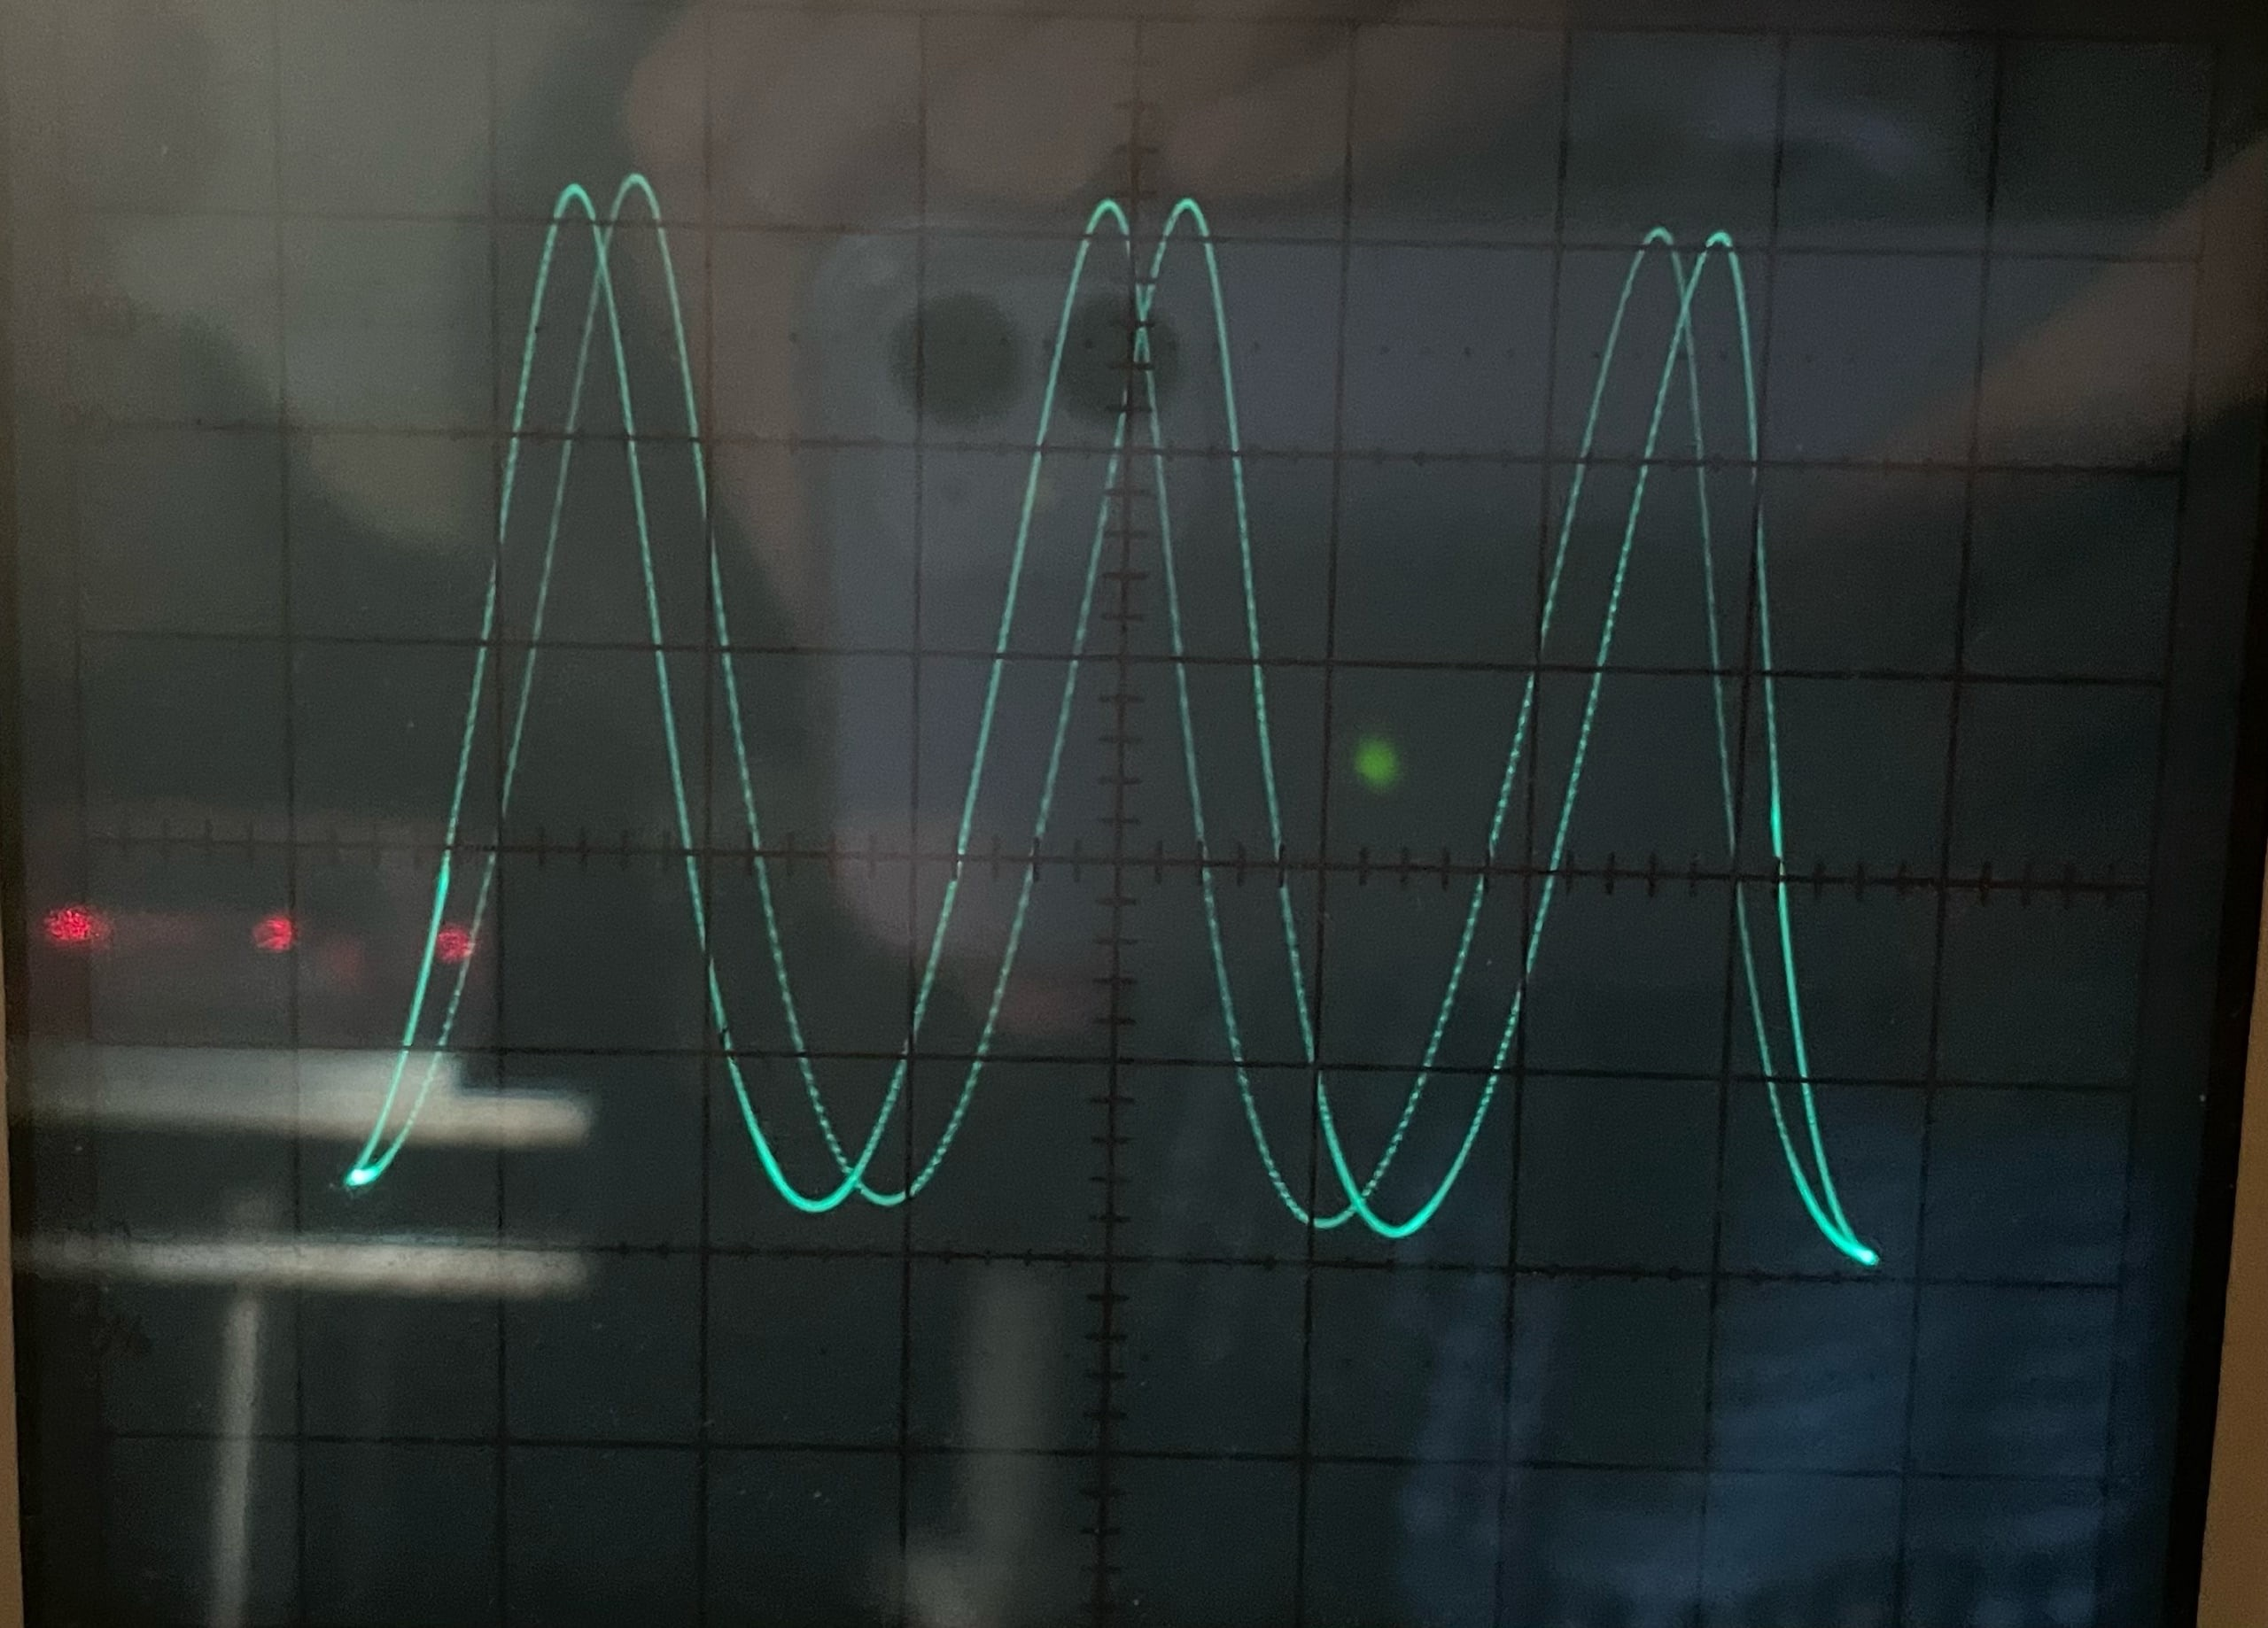
\includegraphics[height=4cm]{liss3.png} \\ \hline
$U_{\lambda/2}$ & $U_{\lambda}$ & $U_{3\lambda/2}$ \\ \hline
\end{tabular}
\caption{Фигуры Лиссажу для различных напряжений}
\label{tab:my-table}
\end{table}

\paragraph{Вывод:} в данной лабораторной работе мы исследовали интерференцию света, прошедшего кристалл. \par
Вычислили $n_0-n_e = 0,102\pm 0,027$. \par
Измеряли полуволновое напряжение кристалла двумя способами, и они совпали в пределах погрешности.

\end{document}
